\documentclass{beamer}
\usetheme{Ilmenau}
\usepackage{amsmath,float,setspace,lmodern,graphicx,amsthm,amsfonts,multirow,hyperref,bm,bbm}

\setbeamertemplate{itemize items}[default]
\setbeamertemplate{enumerate items}[default]

\setbeamercovered{transparent}

\title[Reproducibility with \texttt{git} and \texttt{knitr}]{\texttt{GIT}ting started with reproducibility: \\ An introduction to \texttt{git} and \texttt{knitr}}
\author{Nick Seewald}
\subtitle{Biostatistics Student Association Computing Workshop}
\institute[University of Michigan]{Department of Statistics \\ University of Michigan}
\date{January 29, 2016}
% \logo{\includegraphics[height=.6cm]{blockm.png}}

\begin{document}
	
	\maketitle
	
	\section{Introduction}

	\begin{frame}{Why do I care about reproducibility?}
		Reproducible research is a hallmark of the scientific method, but we're pretty bad at it. 
		
		\begin{quote}
			In 2012, a researcher then at the biotechnology company Amgen wrote in Nature that when his team tried to reproduce 53 landmark cancer studies, they could replicate just six. And according to a news report in Nature, a project aiming to reproduce the findings of 100 psychology papers has managed to replicate results for only 39 of them (the project's findings are still under peer review).
		\end{quote}
		
		\footnotesize{''What Science Can Tell Us About Bad Science'', \textit{The Atlantic}, September 2015.} \scriptsize{\url{http://www.theatlantic.com/magazine/archive/2015/09/a-scientific-look-at-bad-science/399371/}}
	\end{frame}

	\begin{frame}{But I'm a Biostatistician!}
		\begin{itemize}
			\item Reproducibility is important in both science AND statistics!
			\item As statisticians, we need to be able to reproduce our results on the same data set
			\begin{itemize}
				\item This means we have to write reports in a way that minimizes error and write code so that we can get the same results years later.
			\end{itemize}
		\end{itemize}
	\end{frame}
	
	\begin{frame}{Agenda}
		\begin{enumerate}
			\item \texttt{Git}: A ``version control'' tool used for collaborating and maintaining different versions of a file, typically for code.
			\begin{itemize}
				\item Great for collaborating, or just saving your own ass.
				\item Often used in conjunction with \textit{GitHub}, an online repository storage service.
			\end{itemize}
			\item \texttt{knitr}: An R package that lets you create documents containing R code and output.
			\begin{itemize}
				\item Keep everything you need to generate a report (e.g., for research, homework, or 699) in one place!
				\item My favorite part: Update code without having to re-create tables! (This is where errors creep in!)
			\end{itemize}
		\end{enumerate}
	\end{frame}
	
	\section{\texttt{Git}}
	
	\begin{frame}{A Brief Warning}
		\begin{figure}
			\centering
			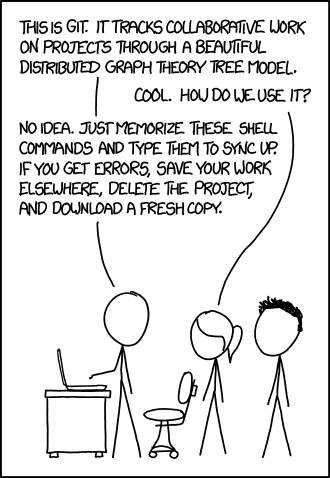
\includegraphics[height=.75\textheight]{xkcd-git.png}
		\end{figure}
		\scriptsize{Source: \url{https://xkcd.com/1597/}}
	\end{frame}
	
	\begin{frame}{Setup}
		Create a GitHub account, then download either Git or GitHub Desktop.
		\begin{itemize}
			\item Pure Git (i.e., just command-line tools): \url{https://git-scm.com/downloads}
			\item GitHub Desktop (GUI \& command-line tools): \url{https://desktop.github.com/}
		\end{itemize}
	\end{frame}
	
	\begin{frame}{\texttt{clone} a Repository}
		\begin{itemize}
			\item To create a local copy of an existing git repository, use 
			\\ \texttt{git clone [url] [directory-name]}.
			\item In a terminal (Mac, Linux) or the Git Shell (Windows), navigate to the folder you want to clone the repository into.
			\item \textbf{Exercise:} Clone my \texttt{bsa-computing} repository onto your computer. The URL is \url{https://github.com/nseewald1/bsa-computing.git}
		\end{itemize}
	\end{frame}
	
	\begin{frame}{Make Changes!}
		\begin{itemize}
			\item You now have a copy of both the current version of \texttt{bsa-computing} \textit{and} access to every previous version.
			\item This clone is NOT automatically synced, \`a la Dropbox
			\begin{itemize}
				\item Anything you break is completely isolated from the pristine copy on GitHub and your previous ``commits''.
			\end{itemize}
			\item \textbf{Exercise:} Add to \texttt{food-exercise.md}, and save your changes.
		\end{itemize}
	\end{frame}
	
	\begin{frame}{Making Commits}
		\begin{itemize}
			\item Once you've accomplished a relatively small, but still significant task, you'll want to ``commit'' your code to the repository.
			\item This creates a labeled snapshot of the directory at the time of the commit.
		\end{itemize}
	\end{frame}
	
	\section{\texttt{knitr}}
	
	\begin{frame}{What is \texttt{knitr}?}
		\begin{itemize}
			\item \texttt{knitr} lets you embed code and output from R into \LaTeX, HTML, RMarkdown, etc.
		\end{itemize}
	\end{frame}
	

\end{document}
